%!TEX program = xelatex
% 完整编译: xelatex -> bibtex -> xelatex -> xelatex
\documentclass[lang=cn,11pt,a4paper,cite=authoryear]{elegantpaper}

\title{论文标题}
\author{周晓龙}
\date{\today}

% 本文档命令
\usepackage{array}
\usepackage{ctex}  %使用宏包(为了能够显示汉字)
\usepackage{datetime}   %使用日期
\usepackage{cite}
\usepackage{fancyhdr}
	\pagestyle{fancy}
	\lhead{ } 
	\chead{ }
	\rhead{\leftmark}
	\lfoot{ }
	\rfoot{ }
\usepackage{lipsum}

\newcommand{\ccr}[1]{\makecell{{\color{#1}\rule{1cm}{1cm}}}}
\renewcommand{\today}{\number\year 年 \number\month 月 \number\day 日}
% \newcommand{\upcite}[1]{\textsuperscript{\textsuperscript{\cite{#1}}}}





\begin{document}

\clearpage
\

% 封面
\begin{figure}[htbp]
  \centering
  
\includegraphics[scale=0.6]{1.jpg}
\end{figure}

\begin{center}
{\heiti \zihao{2} 本科生课程作业}
\end{center} 

\

\begin{figure}[htbp]
  \centering
  
\includegraphics[scale=1.2]{2.jpg}
\end{figure}

\begin{center}
{\heiti \zihao{2} 课程名称}
\end{center} 

\

\begin{center}
{\heiti \zihao{4} 学 \quad \quad 院:\quad \underline{\ \ \ \ \quad 牛牛学院 \quad  \ \ \ \ \ }}

{\heiti \zihao{4} 专 \quad \quad 业:\quad \underline{ \ 测控技术与仪器 \ \ \ }}

{\heiti \zihao{4} 年 \quad \quad 级:\quad \underline{\ \ \ \ \quad \quad 2019 \quad \quad \ \ \ \ \ }}

{\heiti \zihao{4} 姓 \quad \quad 名:\quad \underline{\ \ \quad \quad 我好帅 \quad \quad \ \ \ }}

{\heiti \zihao{4} 学 \quad \quad 号:\quad \underline{\ \ \quad 30192020xx \quad \ \ \ }}

{\heiti \zihao{4} 指导教师:\quad \underline{\ \ \quad \quad 你好帅 \quad \quad \ \ \ }}

\

\

\

\

\

{\heiti \zihao{4} 日期:\quad \today}
\end{center} 
% 封面
\clearpage

\maketitle

% 摘要
\begin{abstract}

MFC压电纤维复合材料是一种新型的智能材料,具有柔韧性和机电
耦合性能好、成本低等优势,在振动能量收集领域具有广阔的应用前景。
然而传统供能方式已无法满足微型化、低功耗器件日常需求,压电振动能量收
集技术为微功耗器件供电提供了新方法。

文章第一部分,介绍了压电效应以及压电传感器、还整体介绍了传统的压电材料以及新型压
电材料种类、特点。

文章第二部分,介绍了基于压电陶瓷的$d_{33}$型MFC的制备工艺,制备流程以
及制备过程中的注意事项,还介绍了以MFC材料制作MFC俘能器的简要过程。

文章第三部分,以$d_{33}$型MFC为例,介绍了MFC的电学性能,主要包括阻抗、介电损耗、谐振频率
三个电学性能,这三个电学性能均可以通过一定的实验手段获得。其中阻
抗和介电损耗可以通过阻抗分析仪获取,谐振频率可以通过正弦激励法获取。


文章第四部分,从激振力、激振频率、结构参数三个方面分析
了MFC材料制作成MFC俘能器的输出特性,其中结构参数方面主要是叉指电极间距对俘能器的输出特性的
影响。另外,这一部分,本文论述了MFC在实际应用中的的负载效应,发现在全波整流电路下,本征电阻
等于负载电阻时,具有最高的输出功率,可以指导MFC俘能器的实际应用。

文章最后对MFC压电材料以及根据MFC材料制作的MFC俘能器进行了总结,并且进行了课程反思,针对
国内传感器领域卡脖子的现象做出了自己的思考,并且根据自己的现有经历,提出了一些可行的解决方案。


\keywords{MFC,新型压电纤维复合材料,能量收集,能量检测}
\end{abstract}
\clearpage

% 目录
\tableofcontents

\clearpage

\section{绪论}

\subsection{压电材料}

压电材料是在压力作用下发生极化而在两端表面间出现电位差的电介质。在
异极晶体材料的特定方向上施加应力,晶体一些对应表面上
分别出现正、负束缚电荷,其电荷密度与施加应力的大小成比例,当应力
反向时,电荷改变符号,这种由机械应力使电介质极化,并形成晶体表面荷电
的效应称为压电效应。

压电材料是明显呈现压电效应的敏感功能材料,为物性型
的,选用合适的压电材料是设计高性能传感器的关键。

常见的压电材料有压电单晶体、压电陶瓷、压电聚合物材
料(PVDF)和压电半导体材料,其各有不同的特点,也有不同
的应用场景。

\subsection{压电复合材料}

随着高新领域的飞速发展和一些特殊性要求,传统
的压电陶瓷因其脆性大、极限应变小、抗机械冲击能力弱等
缺点,使其很难应用于弯曲或者表面不规则区域﹐极大限制了
它在柔性结构方面的应用。而压电聚合物材料虽具有极好的柔性,但
压电性能偏弱,且其应用受温度的影响很大。为了克服上述单相压电
陶瓷的缺点,一种具有新型结构的压电复合材料应运而生。 随着高新领
域的飞速发展和一些特殊性要求,传统的压电陶瓷因其脆性大、极
限应变小、抗机械冲击能力弱等缺点,使其很难应用于弯曲或者表面不规则
区域,极大限制了它在柔性结构方面的应用.而压电聚合物材料虽具有极好
的柔性,但压电性能偏弱,且其应用受温度的影响很大.为了克服上述单相压
电陶瓷的缺点,一种具有新型结构的压电复合材料应运而生。

压电复合材料是指由无机压电陶
瓷和有机高分子树脂按照一定的空
间结构、一定的连通方式复合形成的具有压电效
应的新型材料,它不仅具有优异的压电性能,而且拥
有良好的柔韧性。对于拥有压电陶瓷和有机高分子树脂两种组
分的压电复合材料,根据功能相和聚合物基体的连通方式的不同,可以
将其分为十种基本
类型,分别是 0-0、0-1、0-2、0-3、1-1、1-3、2-1、2-2、2-3和3-3型。在
类型m-n中,m和n分别代表压电功能项和聚合物
基体的连通方式。目前研究较为广泛的类型主要是1-3型和2-2型
压电复合材料,其结构示意图如下所示。


\begin{figure}[htbp]
  \centering
  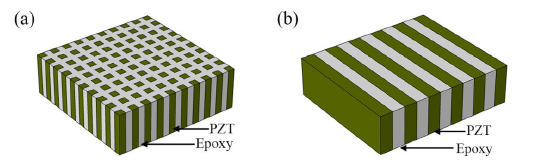
\includegraphics[scale=0.6]{1.png}
  \caption{1-3类型压电材料和2-2型压电材料}
\end{figure}

1-3型压电复合材料在医学超声领域拥有很好
的应用。以1-3型压电复合材料为元件制备的医用超声
探头比无机压电材料更柔软﹐且具有更高的机电耦合系数,灵敏度
显著提高。与1-3型压电复合材料相比,2-2型压电复合材料由于制备
工艺简单、形状参数易于控制、在双组分连接方向上具有良好的自由度等
优点也引起了广泛关注。


\section{压电纤维复合材料}

\subsection{压电纤维复合材料起源}

压电纤维复合材料(Macro Fiber Composite,MFC)是一种新型
结构的智能材料,它是由压电陶瓷纤维、有机聚合物树脂和交叉指型电
极按照一定的空间结构复合形成的。MFC可在密封、耐用的包装中实现面
内极化、驱动和传感[1-3]。

电极以交叉指状的模式喷附在聚酰亚胺薄膜上,从而将施加的
电压传递到压电纤维棒上。如果施加电压,它会弯曲或扭曲材料,抵
消振动,或产生振动。如果不施加电压,它可以作为一个非常敏感的应
变计,感应变形、噪声和振动。MFC也是一种极好的从振动中获取能量的功能材料。

MFC材料是基于美国麻省理工学院最早提出的AFC结
构(Active Fiber composite),并采用挤出成型法制备了柱形压电
纤维胚体,然后高温烧结得到了压电陶瓷纤维,通过叉指电极封装后极化得到
了压电纤维复合材料[4,5]。

\begin{figure}[htbp]
  \centering
  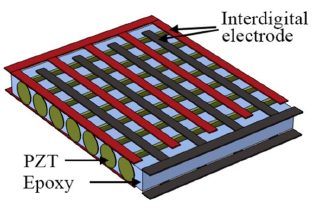
\includegraphics[scale=0.6]{2.png}
  \caption{AFC结构示意图}
\end{figure}

AFC在结构上存在一些弊端[6],即圆柱形压
电纤维和叉指电极的接触面极小,这就导致极化过程
中需要更高的极化电压,且极化电压无法有效的作用在压电纤维上
面,最终导致AFC驱动性能差。挤出成型法制备的压电纤维工艺复杂,容
易发生纤维断裂和排列不整齐的现象,增加了制备成本[7]。
  
为解决上述困难,NASA成功制备了另一种压电纤
维复合材料——MFC(MarcoFiber Composite),其结构和
AFC类似,只是在其基础上将柱状压电纤维替换成截面为矩形的压电
纤维[8]。MFC制备工艺是先采用流延法制备素胚,并通过高温烧结得到压电
陶瓷薄片,然后采用精密划片机切割成尺寸精细且排列整齐的压电纤维
阵列,并利用环氧树脂填充纤维间距形成压电纤维层,最后通过叉指电
极封装即可得到MFC压电纤维复合材料。相较于AFC,MFC中的压电纤维为
截面为矩形,极大的提高了叉指电极和压电纤维的接触面积,极化电压可有效的施
加在压电纤维上,提高了器件的驱动性能。而且MFC的制备工艺更
加简单,易于操作,可重复性强,便于批量化生产。

\subsection{压电纤维复合材料的发展}
目前,应用最广泛的两种结构类型的MFC分别
是$d_{33}$型MFC和$d_{31}$型MFC,如图所示。两者最大的区别
在于极化方向不同。$d_{33}$型 MFC相邻电极的极性相反,即
电极正、负交叉排列,所以其极化方向是沿着压电纤维长度方
向;而$d_{31}$型MFC压电纤维层同侧为同种电极,所以其
极化方向是沿着压电纤维厚度方向。

\begin{figure}[htbp]
  \centering
  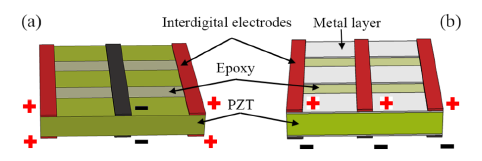
\includegraphics[scale=0.8]{3.png}
  \caption{$d_{33}$型MFC和$d_{31}$型MFC}
\end{figure}

MFC压电纤维复合材料因其独特的结构、优异的传感性能和驱
动性能,在振动主动控制、结构健康监测和能量收集等领域发挥着巨大的作用。

本文主要针对$d_{33}$型MFC材料以及其在振动能量收集领域的应用[9]。

\section{$d_{33}$型MFC的制备}
\subsection{材料选择}

\subsubsection{压电陶瓷}

MFC制备所用到的材料主要为压电陶瓷
材料、聚合物、柔性叉电极,下文针对
这三种材料的选择进一步论述。

压电材料的性能参数决定了压电器件的发电性能。压电
发电器件应该选择压电常数高、相对介电常数大、机械品质
因数高的压电材料。根据研究对比当前应用较广的压电陶瓷,本文采用
压电常数较高的PZT-5H压电陶瓷,其主要性能参数如下:
\begin{figure}[htbp]
  \centering
  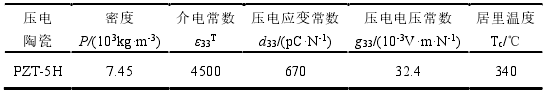
\includegraphics[scale=0.9]{4.png}
  \caption{压电陶瓷的主要性能参数}
\end{figure}

\subsubsection{聚合物}
压电陶瓷因脆性大的特点而限制了其在曲面的应
用,因此通过引入聚合物,使压电陶瓷和聚合物
复合得到压电复合材料,从而拓展了压电器件的应用领
域。环氧树脂是一种热固性高分子聚合物﹐当它与固化剂进行
固化反应形成三维交联网络结构后,则呈现出一系列优良的特性,如力
学性能好、粘结性能优异、固化收缩较小、稳定性高等。

\subsubsection{柔性叉指电极}
柔性叉指电极(F1exible Printed Circuit,FPC),是通过
电化学工艺加工获得的具有指状或梳状周期性图案电极的超精细电路,其
基底材料为绝缘性能好,介电损耗低,稳定性高且与铜箔有很好
匹配性的聚酰亚胺膜。

作为一种特殊的电路板﹐FPC的制备工艺使其具有了得天独
厚的优势:可以自由弯曲、卷绕、折叠,可依照空间布
局要求任意安排,并在三维空间任意移动和伸缩,从而达到元器件装
配和导线连接的一体化;利用FPC可大大缩小电子产品的体积和重量,适用电
子产品向高密度、小型化、高可靠方向发展;FPC还具有
良好的散热性和可焊性以及易于装连、综合成本较低等优点,软硬结
合的设计也在一定程度上弥补了柔性基材在元件承载能力上的略微不足。


\subsection{制备流程}
MFC压电纤维复合材料的制备流程如下图所示:
\begin{figure}[htbp]
  \centering
  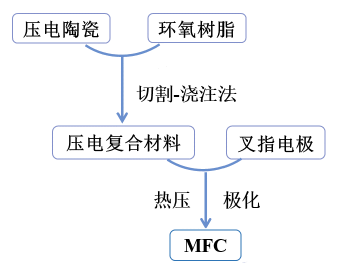
\includegraphics[scale=0.5]{5.png}
  \caption{MFC制备流程}
\end{figure}

制备主要的流程包括陶瓷纤维的切割、2-2型压电复合材料的制备、MFC压电复合材
料的封装和极化。由于所制备的陶瓷纤维厚度薄且宽度小,制备过程
中易出现纤维断裂、浇注成型困难等问题,根据已
有研究[8],可从以下几个方面改进了制备技术:

\begin{enumerate}
  \item 通过精密划片机切割厚度均匀的压电陶瓷纤维,以确保纤
  维的细小尺寸、均匀厚度和有序排列;
  \item 改进浇注成型技术,确保得到平整的2-2型压电复合材料;
  \item 通过热压的方法实现MFC封装,确保
  电极和纤维层的有效接触,有利于后续MFC的极化和电输出性能的测量。
\end{enumerate}

进行制备时,常见的作法是,首先使用精密划片机对
压电陶瓷进行切割,制备得到压电陶瓷纤维。

当具备了压电陶瓷纤维之后,将环氧树脂和固化
剂按照质量比4:1混合,充分搅拌均匀后放置于真空泵中,抽真空
5min去除基体中存在的气泡,直至树脂表面无微小气泡冒出。从压
电纤维层的一侧,利用环氧树脂的高流动性使其填充满陶瓷纤维
间隙,然后去除纤维表面多余的树脂,随后放入真空泵中抽真空2min后
静置12h,等待环氧树脂固化;待环氧树脂彻底固化后,去除底面的UV膜即
得到压电纤维层。

最后,按照如下步骤,调整纤维层和铜
电极区域,并进行热处理,完成对纤维材料进行封装。


\subsection{极化}

MFC压电纤维复合材料的核心是压电陶瓷,未极化的
压电陶瓷其内部电畴呈现杂乱无章的排列方式,没有压
电性。极化的目的就是对压电陶瓷施加直流电压,使得
陶瓷内部电畴沿着电场方向偏转,形成单向电畴结构,最常
用的就是采用油浴极化法对MFC进行极化。

极化时候需要注意如下几点:

\begin{enumerate}
  \item 极化电场
  
  电场越强,促使铁电畴定向排列的效果越好,极化效果就越好;

  \item 极化温度
  
  在确定的极化电压和时间下,极化温度高,电畴取向排列的程度高,极化效果好;
  \item 极化时间
  
  极化时间长,电畴取向排列的程度高,极化
  效果好,极化初期主要是$180^{\circ}$电畴的转向,之后是$90^{\circ}$电
  畴的转向,但$90^{\circ}$
  电畴转向油浴内应力的阻碍而较难进行,因而适当
  增加极化时间,可增强极化效果;
  \item 材料缺陷
  
  如压电纤维层中聚合物基体中存在
  气泡,当施加较大直流电压时,会因气泡中空气的
  存在而产生电击穿,因此在压电纤维层的制备和封装过程,要尽可
  能的除去环氧基体中的气泡。
\end{enumerate}

\section{MFC的性能}
\subsection{电学性能}
\subsubsection{阻抗}
MFC的阻抗为MFC在电路中对电流的阻碍作用,用$Z$表示,有:

$Z = R + jX$

其中,$R$为电阻,$X$为电抗,$X = wL - \frac{1}{wC}$, $wL$为
感抗,$\frac{1}{wC}$为容抗。

最常用测量MFC的阻抗方法就是使用阻抗分析仪,此时有:

\begin{equation*}
  Z = \sqrt{R^2 + X^2}
\end{equation*}


\subsubsection{介电损耗}
介电损耗D是所有介质材料的重要品质
指标之一,通常使用$tan\delta$来表示介质损耗,也称为损耗因子:
\begin{equation*}
  tan\delta = \frac{1}{wCR}
\end{equation*}

式中,$o$是交变电场的角频率,$C$为介质电容,$R$为损耗
电阻。处于交变电场中的介电损耗是由于介质材料电导过程和极化弛
豫引起的,而且对于具有铁电性的压电陶瓷而言,介电损耗还和畴壁的运动有关。


\subsubsection{谐振频率}

MFC属于振荡机械系统,其谐振频率是由陶瓷刚度和有效
质量决定的。实际谐振频率测量方法为:对MFC施加交变电
压信号激励,当激励信号的频率与压电陶瓷的固有频率接近的
时候,发生共振现象,此时,MFC的阻抗最小,此时的振荡频
率即为MFC的谐振频率。


\section{MFC俘能器性能分析}

在MFC应用于在振动能量收集领域时,其结构参
数和性能是非常重要的。本节主要论述激振频率
和激振力对MFC俘能器的性能影响[10]。

\subsection{激振力对MFC俘能器的输出影响}
激振力在高频振动状态下难以直接获得,因此利用加速度
传感器来测量振动实时加速度,从而间接的求解出激振
力的大小。下图显示了六种加速度下俘能器的最大开路电压和
取得的最大电压时的振动频率。

\begin{figure}[htbp]
  \centering
  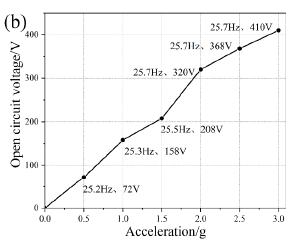
\includegraphics[scale=0.7]{6.png}
  \caption{激振力对输出特性的影响}
\end{figure}

从图可以看出,随着振动加速度的增加,MFC俘能器所
产生的最大开路电压呈逐渐增大的趋势。而且振动加速
度对俘能器的电输出性能影响非常大,从图中可以明
显看出,当振动加速度为0.5 g时,俘能器的最大开路
电压为72 V;而当加速度增加至2g 时,其最大电压为320 v,与72V相比
增加了3.4倍;当加速度为3g时,俘能器开路电压较与72V相比增加了4.7倍。从图
中还可以看出,当加速度从0.5 g 增加至2g时,俘能器的共振频率
逐渐增大,加速度大于2g后,其共振频率趋于稳定。

此外,当加速度为0.5g时,MFC俘能器自由
端的振幅小,因此所产生的开路电压偏小,而当加
速度增加时3g时,在其谐振频率下自由端的振幅过大,不适合长
时间可靠工作。综合考虑,选择2g
的固定加速度,在此加速度下,既能满足MFC俘能
器产生足够大的开路电压,又能保证其可靠性。

\subsection{激振频率对MFC俘能器的输出影响}

自然界的振动往往以低频为主,因此本文主要研究低频
条件下MFC俘能器的电输出性能。设置振动加速度为2g,研
究激振频率对MFC俘能器电输出性能的影响,结果如图所示[11]。

\begin{figure}[htbp]
  \centering
  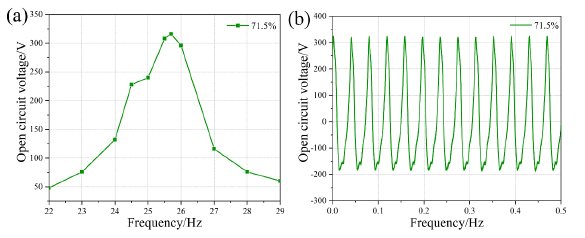
\includegraphics[scale=0.7]{7.png}
  \caption{MFC俘能器频域响应}
\end{figure}

由此可见,俘能器的开路电压对振动频率的响应非常敏感,因此在压
电振动能量收集的实际应用中,应该尽可能的选择振动频率和装
置共振频率相一致,如此才可获得更大开路电压。


\subsection{结构参数对MFC俘能器的输出影响}
\subsubsection{叉指电极间距对俘能器输出性能的影响}

在三种间距下的MFC俘能器在谐振频率下得到的电压:

\begin{figure}[htbp]
  \centering
  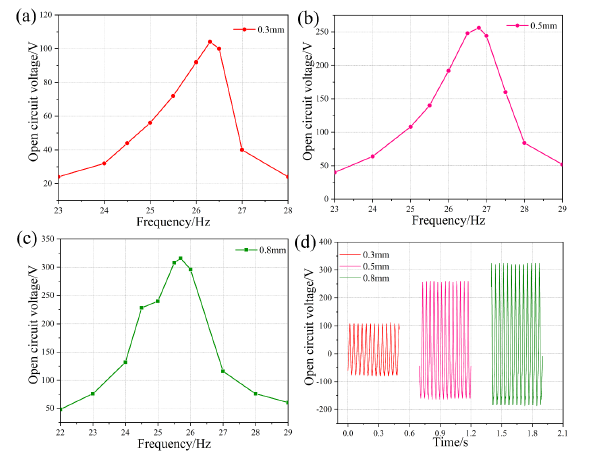
\includegraphics[scale=0.7]{8.png}
  \caption{电极间距对MFC的输出电压的影响}
\end{figure}

三种MFC俘能器的输出电压均随着频率增加呈现先增大后减小
的趋势,在其共振频率处,俘能器的最大输出电压随
着叉指电极指间距的增大而逐渐增大。

\subsection{MFC的负载响应}

试验阶段,MFC俘能器的电输出特性主要是通过开路
电压表征,实际应用中,俘能器需要配合负载一
起使用,所以研究MFC的负载特性非常重要。
  
下图为MFC俘能器的负载测试示意图,主要包括俘能器的
振动系统、整流桥、负载电阻、示波器。俘能器所产生的电压为正
弦交变电压,而整流桥的作用是将电路中的交流电转换为直流电,这是通过二极
管的单向导通原理来完成的。
  
整流电路的类型主要有半波整流、全波整流和桥式
整流三种。其中半波整流是利用二极管的单向导通性,输出所获得正弦
电压的正半部分,而负半部分则损失掉;与半波整流方式相比,全波整流所获
得的正弦电压的正半部分信号保持不变,而负半部分的信号全部反向,从而得
到连续的电压信号,故采用全波整流的方式。

下图即为MFC的负载特性:
\begin{figure}[htbp]
  \centering
  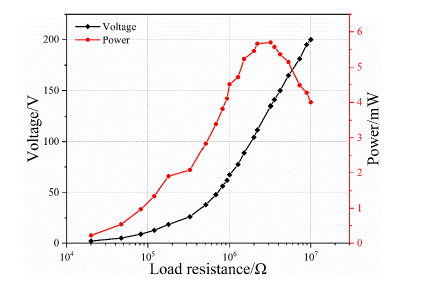
\includegraphics[scale=0.7]{9.png}
  \caption{MFC的负载特性}
\end{figure}

MFC的功率由以下公式计算得出:

\begin{equation*}
  P = \frac{rU^2}{(r+R)^2}
\end{equation*}

其中,$P$为俘能器的输出功率,$U$是俘能器产生的总电压,$r$为负载电阻,$R$为MFC电阻。

根据负载特性曲线, MFC俘能器的输出功率随着负载电阻的增大而呈现
先升高后降低的趋势。当负载电阻为3.2 MQ时,俘能器输出功率达到最大值,为5.70 mW。当
功率对负载电阻r求导可得:

\begin{equation*}
  \frac{dP}{dr} = \frac{(R-r)U^2}{(R+r)^2}
\end{equation*}

当$r=R$时,$P'=0$,MFC俘能器的输出
功率取得最大值。因此可以得出,MFC俘能
器的输出功率与负载电阻有极大关系,而且最优负
载阻值和MFC压电纤维复合材料有关。在实际应用中,为获
取更大的输出功率,应选择合适的负载电阻。


\section{MFC材料的其它应用}

\subsection{MFC在振动控制中的应用}

振动主动控制是指在振动控制过程中,根据所检测
到的振动信号,应用一定的控制策略,经过实时计算,进而驱
动作动器对控制目标施加一定的影响,达到抑制或消除振动的
目的。如飞机、航天器、船等工作时,因振动和噪声激起的振动响应
可能会造成结构破坏、承力件断裂等后果,因此采用驱动器进行
振动主动控制,从而实现抑制或消除振动具有重要的意义。
  
MFC因其质轻、柔韧性好、灵敏度高且能量密度大等特点,在结构振动
主动控制领域显示出极大的优越性。Sohn等人[12]在船体结构上
应用了压电纤维复合材料,研究发现MFC可以有效的提高船体的减振
效果。此外,MFC因其灵活的驱动指向性,可以明显增强扭转驱动效果,在航空
航天领域的振动主动控制方向具有极好的应用前景。如Paradies等人[13]采用MFC阵列
实现了对无人机机翼的转动控制。

\subsection{MFC在结构健康检测的应用}

结构健康监测是近些年国内外研究热点。如桥梁、管道等长
期服役的结构可能因环境温湿度等自然或人为因素的作用,造成结构疲劳
效应和结构损伤,甚至引发突然性破坏。因此对桥梁、管道等结
构进行健康监测,确保其安全运营具有重要意义。MFC压电纤维
复合材料作为一种非常敏感的应变传感器,可灵敏的感知低频振
动信号,而且还具有优异的柔性,可以弯曲以很好地匹配曲面结
构的曲率,因此可应用于桥梁、管道等结构的健康监测。如Lin Cui[14]等人利用
压电纤维复合材料产生扭转波对圆柱结构进行健康监测,结果表明,利用该
方法不仅可以监测裂纹出现,而且可以监测裂纹大小和扩展
情况。Seunghee Park等人[15]提出了一种基于MFC阻抗的无线结构健康监测系
统在铁路轨道损伤检测中的异常值分析方法。

\subsection{MFC在振动能量收集领域的应用}
机械振动能普遍存在于我们的日常生活中,诸如
高速公路、城市道路因车辆和行人的运动而产生的
振动能,工厂中发动机的连续振动,甚至是人体心跳、脉搏跳
动振动能量等。所以如何将机械振动能有效的转化为电能具有较高
的研究价值。相较于压电陶瓷器件,MFC压电纤维复合因具有良好的柔韧性和
较大的应变能力,更能有效的收集环境中振动能量并转换为
电能,通过管理电路将能量储存起来,为微机电系统供电[16-18]。


\section{总结}

本文主要针对PZT-5H压电陶瓷制备的$d_{33}$型MFC
压电纤维复合材料进行了研究与论述,并在MFC的振动能量收集领域,对其微
观结构、力学性能和电学性能进
行了分析表征。根据其它学者设计的悬臂梁式MFC俘能器,研究了激振
源(频率和加速度)、结构参数等对MFC俘能器电输出性能的影响。

最终,本文论述了MFC压电纤维复合材料传感器的其它应用,总结了MFC
的应用场景及特点。



\section{课程思考}
目前,国内传感器领域已经得到了长足的发展,但不可否
认的是,国内传感器和国外传感器的研究还有很大的差




\clearpage

\begin{thebibliography}{99}  

  \bibitem{ref1}陈子琪,朱松,林秀娟,熊威,周科朝,张斗.纤维厚度和体积分数对压电纤维复合物应变性能的影响[J].无机材料学报,2015,30(06):571-575.
  \bibitem{ref2}耿学仓,李明轩.检测超声换能器用1-3型压电PZT/环氧复合材料及换能器的研究[J].应用声学,1991(05):10-14.
  \bibitem{ref3}沈辉. 基于压电材料的振动能量回收电路及其应用研究[D].南京航空航天大学,2010.
  \bibitem{ref4}Bent A A, Hagood N W. Piezoelectric fiber composites with interdigitated electrodes[J].Journal of Intelligent Materia1 Systems and Structures,1997,8(11): 903-919.
  \bibitem{ref5}Bent A A,Hagood N W. Rodgers J P. Anisotropic actuation with piezoelectric fiber composites[J]. Journal of Intelligent Material Systems Structures,1995,6(3): 338-349.
  \bibitem{ref6}Paradies R, Melnykowy cz M. Numerical stress investigation for piezoelectric elements with acircular cross section and interdgitated electrodes[J]. Joumal of Intelligent Mat erial Systems Structures, 2007,18(9): 963-972. 
  \bibitem{ref7}Lin X, ZhouK,Button T W, et a1.Fabni cation , characterization, and modeling of piezoelectric fiber compo sites[J].Journal of Appli ed Physics, 2013,114(2):027015.
  \bibitem{ref8}Schulz M J, Sundaresan M J,Ghosha1 A, et al. Active fiber composites for structural healthmonitoring[C]. Smart Structurcs and Matcrials, 2000,3992:13-24.
  \bibitem{ref9}孙杰,黄庭轩,孙禄君,朱东方,黄静.基于压电纤维复合材料的抖振主动控制研究[J].机械强度,2020,42(04):770-776.DOI:10.16579/j.issn.1001.9669.2020.04.002.
  \bibitem{ref10}Park S, Inman D J, Yun C B.An outli er analysis of MFC-based imp edance sensing data for wireless structural health monitoring of railroad tracks[J]. Engineering Structures,2008,30(1 0): 2792-2799.
  \bibitem{ref11}孙亚飞,杨延鹏.悬臂粱微型压电自发电系统研制[J].电子技术与软件工程,2020,000(002):210-212.
  \bibitem{ref12}Sohn J W, Choi S B,Kim H S.Vibration contro1 of smart hull structure with optimally placed piezoelectriccompositeactuators[J]. International Journal ofMechanical Sciences,2011,53(8): 647-659.
  \bibitem{ref13}Paradies R,Ciresa P.Active wing design with integrated flight contro1 using piezoelectric macro fiber composites[J]. Smart Materials Structures,2009,18(3): 035010.  
  \bibitem{ref14}吴学林.桥梁健康监测系统构成及发展[J]﹒南方农机,2018,49(14): 112-112.
  \bibitem{ref15}Park S, Inman D J,Yun C B.An outli er analysis of MFC-based impedance sensing data for wireless structural health monitoring of railroad tracks[J]. Engineering Structures,2008, 30(10): 2792-2799.  
  \bibitem{ref16}Ju s, Chae S H, Choi Y, et a1. Macro fiber composite-based low frequency vibration energyharvester[J]. Sensors A ctuators A: Phy si ca1, 2015,226: 126-136.
  \bibitem{ref17}王海清,刘龙建,胡利民,孙斌,余世科,李皓.基于压电纤维复合材料的洋流能发电装置发电性能分析[叮.电机与控制应用,2020,47(09): 97-105.
  \bibitem{ref18}王红艳,谢涛,王志彬.压电纤维复合材料悬臂梁发电性能分析[J].传感器与微系统,2010(O3): 52-55.

  % \bibitem{ref1}
  % \bibitem{ref2}
  % \bibitem{ref3}
  % \bibitem{ref4}
  % \bibitem{ref5}
  % \bibitem{ref6}
  % \bibitem{ref7}
  % \bibitem{ref8}
  % \bibitem{ref9}
  % \bibitem{ref10}
  % \bibitem{ref11}
  % \bibitem{ref12}
  
\end{thebibliography}


\end{document}



